%%%%%%%%%%%%%%%%%%%%%%%%%%%%%%%%%%%%%%%%%%%%%%%%%%%%%%%%%%%%%%%%%%%%%%%%%%%%%%%%
%                                  FrontPage                                   %
%%%%%%%%%%%%%%%%%%%%%%%%%%%%%%%%%%%%%%%%%%%%%%%%%%%%%%%%%%%%%%%%%%%%%%%%%%%%%%%%

\pagenumbering{gobble}
\newgeometry{top=7cm, bottom=7cm}

\begin{center}
{\fontsize{35}{42} \textsc{Note di calcolabilità}}\\
\vspace{10pt}
\Large{\faGithubAlt\ \texttt{matteogiorgi.github.io}}\\
\vspace{5\baselineskip}
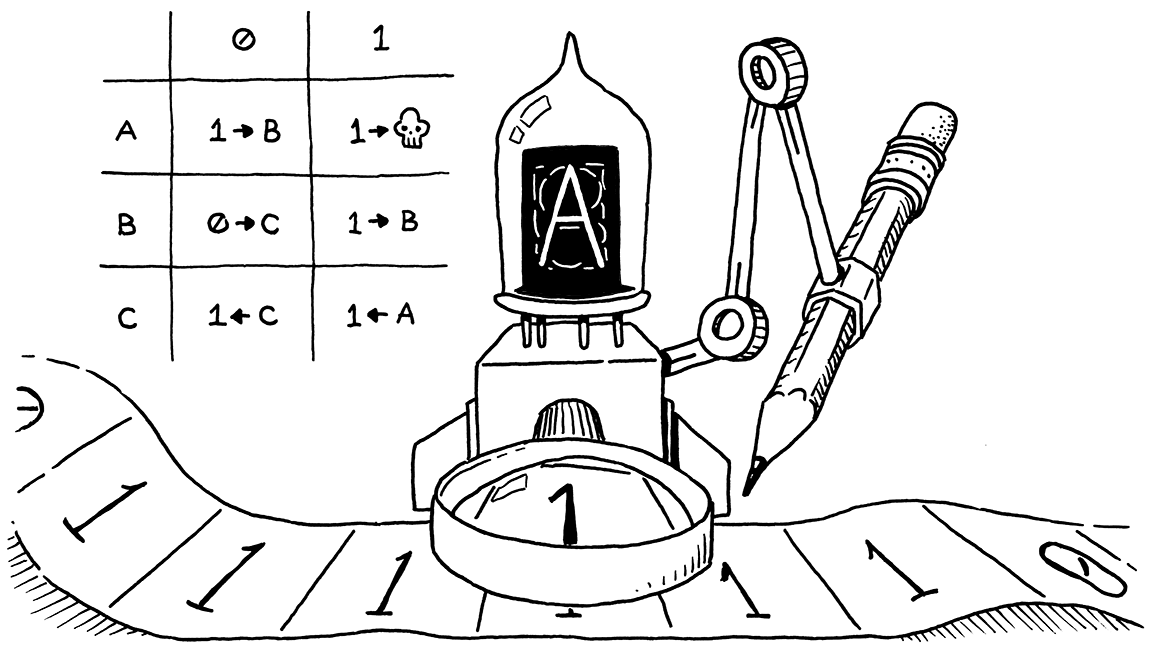
\includegraphics[width=0.9\textwidth]{../assets/machine.png}\\
\vfill
\begin{equation*}
\Large{\texttt{> UniPi 20} \pointer{\texttt{2}}
\texttt{0 \#\#}}
\end{equation*}
\end{center}








%%%%%%%%%%%%%%%%%%%%%%%%%%%%%%%%%%%%%%%%%%%%%%%%%%%%%%%%%%%%%%%%%%%%%%%%%%%%%%%%
%                                  Abstract                                    %
%%%%%%%%%%%%%%%%%%%%%%%%%%%%%%%%%%%%%%%%%%%%%%%%%%%%%%%%%%%%%%%%%%%%%%%%%%%%%%%%

\newpage
\restoregeometry
\addtolength{\topmargin}{20pt}
\pagenumbering{roman}
\renewcommand{\abstractname}{Info\ \faPencil}

\begin{abstract}
Queste note sono state redatte dal sottoscritto durante le lezioni del corso
di \textit{Elementi di calcolabilità e complessità} tenute dal prof. Pierpaolo
Degano, con l'ausilio del dott. Giulio Masetti, per il Corso di Laurea in
Informatica.

Il materiale usato per la stesura, oltre alle note distribuite dal professore,
comprende, in maniera più o meno estensiva, riferimenti ai seguenti testi

\begin{itemize}[itemsep=-7pt]
\item \textit{Sipser - Introduction to the theory of computation}
\item \textit{Taylor - Models of computation and formal languages}
\item \textit{Cutland - Computability, introduction to recursive
    function theory}
\item \textit{Cooper - Computability theory}
\item \textit{Bernasconi, Codenotti - Introduzione alla complessità
    computazionale}
\item \textit{Ausiello, D'Amore, Gambosi - Linguaggi, modelli, complessità}
\end{itemize}
\end{abstract}








%%%%%%%%%%%%%%%%%%%%%%%%%%%%%%%%%%%%%%%%%%%%%%%%%%%%%%%%%%%%%%%%%%%%%%%%%%%%%%%%
%                               Table of Contents                              %
%%%%%%%%%%%%%%%%%%%%%%%%%%%%%%%%%%%%%%%%%%%%%%%%%%%%%%%%%%%%%%%%%%%%%%%%%%%%%%%%

\newpage
\tableofcontents








%%%%%%%%%%%%%%%%%%%%%%%%%%%%%%%%%%%%%%%%%%%%%%%%%%%%%%%%%%%%%%%%%%%%%%%%%%%%%%%%
%                                 Page Numbering                               %
%                                 Page Style                                   %
%%%%%%%%%%%%%%%%%%%%%%%%%%%%%%%%%%%%%%%%%%%%%%%%%%%%%%%%%%%%%%%%%%%%%%%%%%%%%%%%

\newpage
\pagenumbering{arabic}
%\setcounter{page}{0}

\pagestyle{fancy}
\fancyhf{}
\fancyhead[L]{\scshape\faBookmarkO}
\fancyhead[C]{\scshape\leftmark}
\fancyhead[R]{\scshape\thepage}
%\fancyfoot[C]{\thepage}

\renewcommand\chaptermark[1]{\markboth{#1}{}}
\renewcommand\sectionmark[1]{\markright{#1}}
\renewcommand{\headrulewidth}{.5pt}

